\documentclass[12pt,titlepage]{article}

\usepackage[utf8]{inputenc}
\usepackage{ctex}
\usepackage[colorlinks,allcolors=blue,pdflang=zh-CN]{hyperref}
\usepackage{graphicx}

\newcommand{\systemname}{志愿服务信息管理系统}
\newcommand{\systemversion}{v1.4.1}
\newcommand{\githuburl}{https://github.com/huang2002/volunteer-system}
\newcommand{\issuesurl}{\githuburl/issues}
\newcommand{\releasesurl}{\githuburl/releases}
\newcommand{\Python}{\textit{Python}}
\newcommand{\GitHub}{\textit{GitHub}}

\NewDocumentEnvironment{warnings}{b}{%
    \vspace{5ex}
    \noindent
    \begin{minipage}{\linewidth} \itshape
        注意:
        \begin{itemize}
        #1
}{%
        \end{itemize}
    \end{minipage}
    \vspace{2ex}
    \ignorespacesafterend
}

\title{\systemname\\使用手册\\\systemversion}
\author{hhh}

\begin{document} \sloppy

\maketitle

\tableofcontents
\thispagestyle{empty}
\setcounter{page}{0}

\pagestyle{headings}

\newpage
\section{使用指南}

\subsection{软件概述}

\textit{\systemname}是一款由个人开发的免费、开源\footnote{GitHub地址:\url{\githuburl}}
软件,用于录入、保存、整理和统计志愿服务信息。目前,软件以压缩包形式在\GitHub上发布。
\footnote{GitHub Releases: \url{\releasesurl}}

\subsection{软件结构}

解压后,应得到如下软件结构:

\begin{verbatim}
/path/to/volunteer-system
        ├─ backend/
        ├─ frontend/
        ├─ aliases.json
        ├─ 初始化(Windows).bat
        ├─ 初始化(MacOS或Linux).bash
        ├─ 启动(Windows).bat
        ├─ 启动(MacOS或Linux).bash
        ├─ 使用手册.pdf
        ├─ LICENSE.txt
        └─ requirements.txt
\end{verbatim}

其中,

\begin{itemize}
    \item \texttt{frontend}和\texttt{backend}分别存放前端和后端的代码。
    \item \texttt{aliases.json}是用于存放别名的数据文件。
    \item \texttt{*.bat}和\texttt{*.bash}是辅助使用的脚本程序。
    \item \texttt{使用手册.pdf}就是此文档的文件。
    \item \texttt{LICENSE.txt}和\texttt{requirements.txt}分别是开源许可证和\Python依赖项清单。
\end{itemize}

首次成功运行后,会额外生成三个文件夹:\texttt{data}、\texttt{backup}和\texttt{export},
分别用来存放原始数据、备份数据和导出数据。

\subsection{安装\Python}
\label{sec:install-python}

系统后端使用\Python\footnote{Python官网:\url{https://www.python.org/}}语言编写,
使用时需要\Python的解释器程序。因此,使用前需要先安装\Python环境。
如果您的电脑上已经安装了\Python环境,可以跳过此步骤、直接尝试初始化。

\Python官网下载页面:\url{https://www.python.org/downloads/}。
软件开发使用的是\textit{Python 3.9.2},因此建议下载、安装\textit{3.9.X}版本。
安装时,必须要勾选“将\Python添加到环境变量”(Add Python to environment variables)。
安装完成后,可以在命令行窗口或终端执行以下命令:

\begin{verbatim}
python --version
\end{verbatim}

如果正确显示了版本号(例如:\texttt{Python 3.9.2}),则说明安装成功。
否则,说明安装失败或未将\Python添加到环境变量,
请重新安装或着手动将\Python添加到环境变量,具体步骤麻烦自行搜索。

\subsection{初始化}

首次使用前,需要先安装\Python(参考章节\ref{sec:install-python}),并对软件进行初始化。
通常,成功安装\Python后,直接运行系统对应的初始化脚本即可:

\begin{itemize}
    \item \textbf{Windows:} \texttt{初始化(Windows).bat}
    \item \textbf{MacOS或Linux:} \texttt{初始化(MacOS或Linux).bash}
\end{itemize}

运行初始化脚本会打开命令行窗口,自动设置\Python虚拟环境并安装依赖项。
安装成功后,会输出“Initialization finished successfully!”。
无论成功与否,程序结束都应该会有“按任意键继续……”或“Press any key to continue...”,
此时按下键盘上任意字符即可退出,也可直接关闭窗口。

初始化过程中会自动生成\texttt{.venv}文件夹,存放\Python虚拟环境相关文件。
当\texttt{.venv}已经存在时,初始化脚本会跳过初始化直接结束。
如果初始化遇到问题,可以尝试删除\texttt{.venv}文件夹后重试。

\subsection{启动程序}

初始化成功后,运行系统对应的启动脚本即可开始使用本系统:

\begin{itemize}
    \item \textbf{Windows:} \texttt{启动(Windows).bat}
    \item \textbf{MacOS或Linux:} \texttt{启动(MacOS或Linux).bash}
\end{itemize}

运行启动脚本时,会自动打开一个命令行窗口,其中显示的是后台程序的输出。
同时,会尝试启动浏览器并打开系统的前端页面。
如果没有成功打开浏览器,请手动打开浏览器,访问命令行窗口中显示的网址。
(例如:\nolinkurl{http://127.0.0.1:2023}。具体端口可能不同。)

如果不想启动时自动打开浏览器窗口,可以手动修改启动脚本,
给后台程序添加参数\texttt{--no-open}。

\subsection{使用系统}

成功启动后台程序并访问前端页面后,即可开始使用本系统的各项功能。
有关功能介绍,请参考章节\ref{sec:functionalities}。

\subsection{退出系统}

在系统前端页面的右上角,设有“退出系统”按钮。
点击此按钮或直接关闭后台程序的命令行窗口即可停止后台程序,但是前端页面需要手动关闭。

\newpage
\section{功能介绍}
\label{sec:functionalities}

系统的前端页面左侧设有导航菜单,点击菜单中的选项即可打开对应的功能页面。

\begin{figure}[htbp]
    \centering
    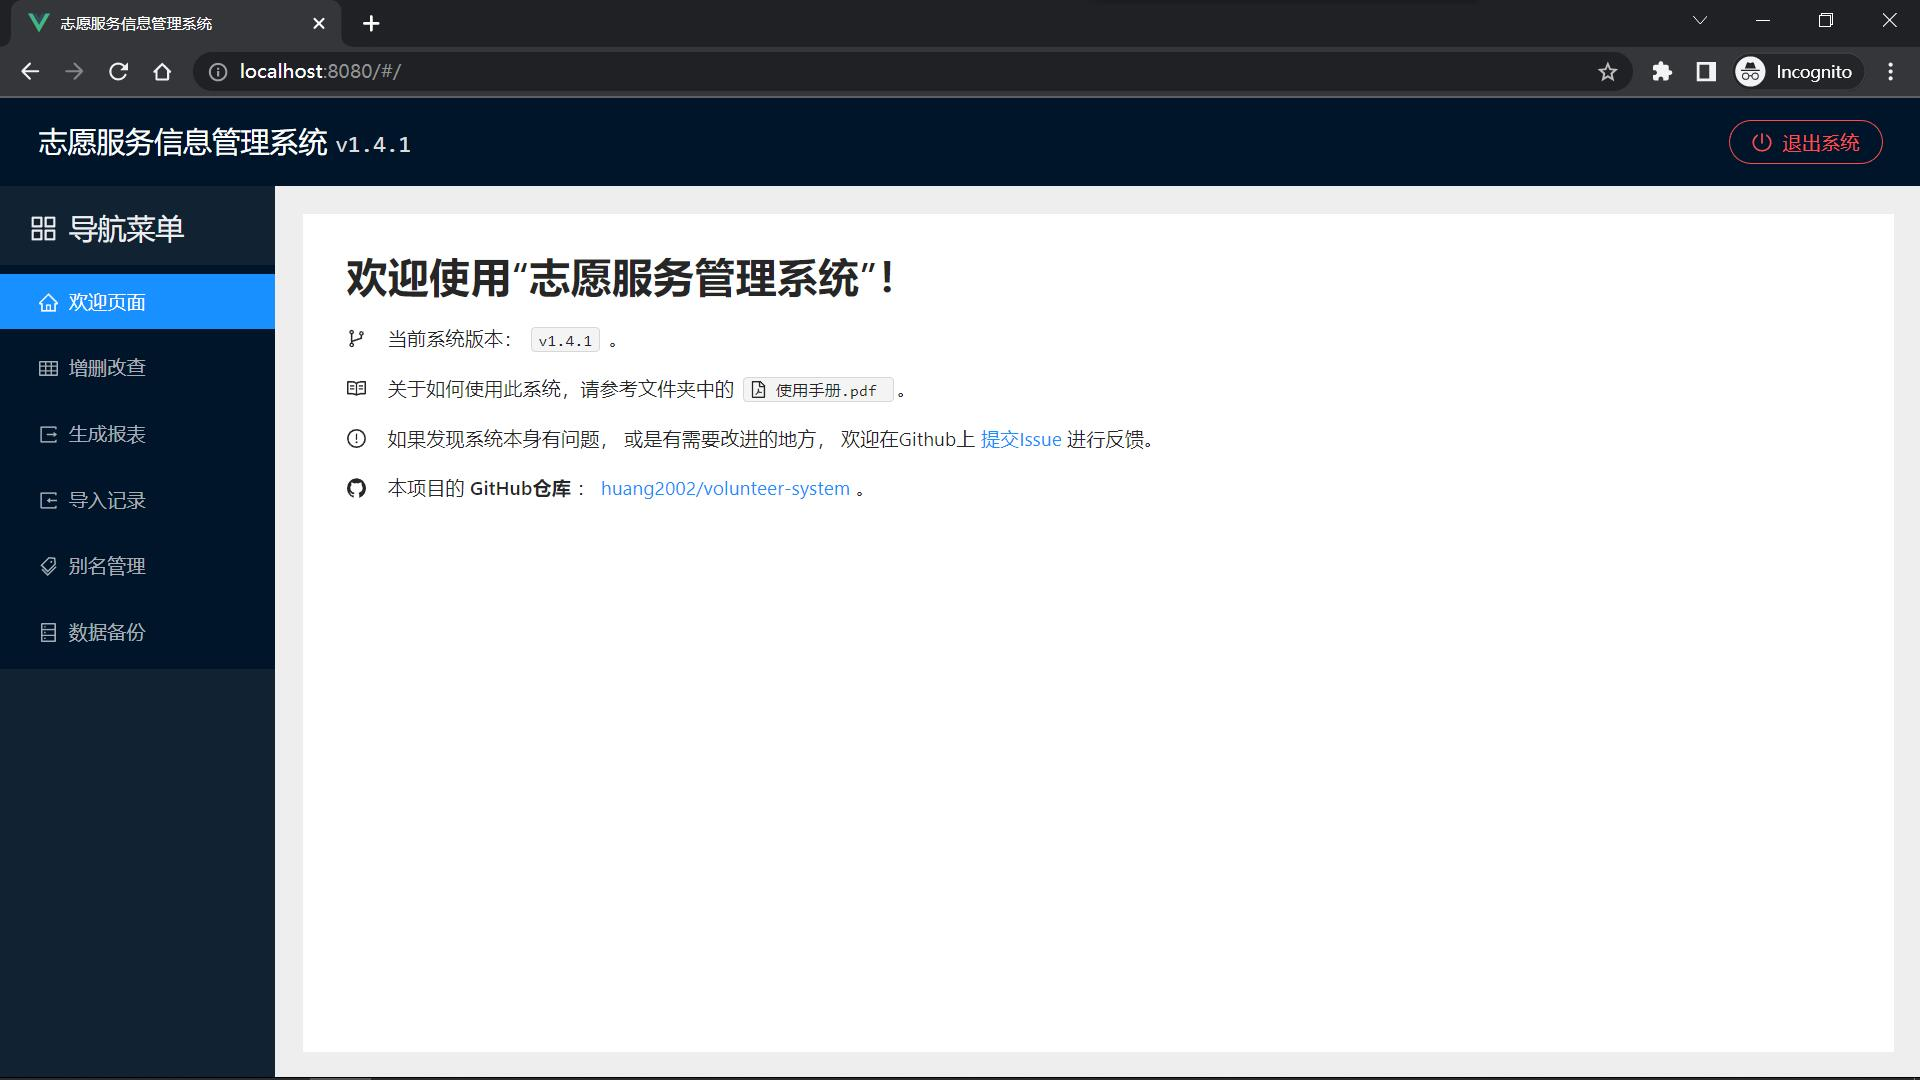
\includegraphics[width=\textwidth]{../screenshots/home.jpg}
    \caption{欢迎界面}
\end{figure}

\subsection{增删改查}

在“增删改查”页面中,可以查看系统中现存表格的所有记录,并进行添加、修改、删除等操作。

\begin{figure}[htbp]
    \centering
    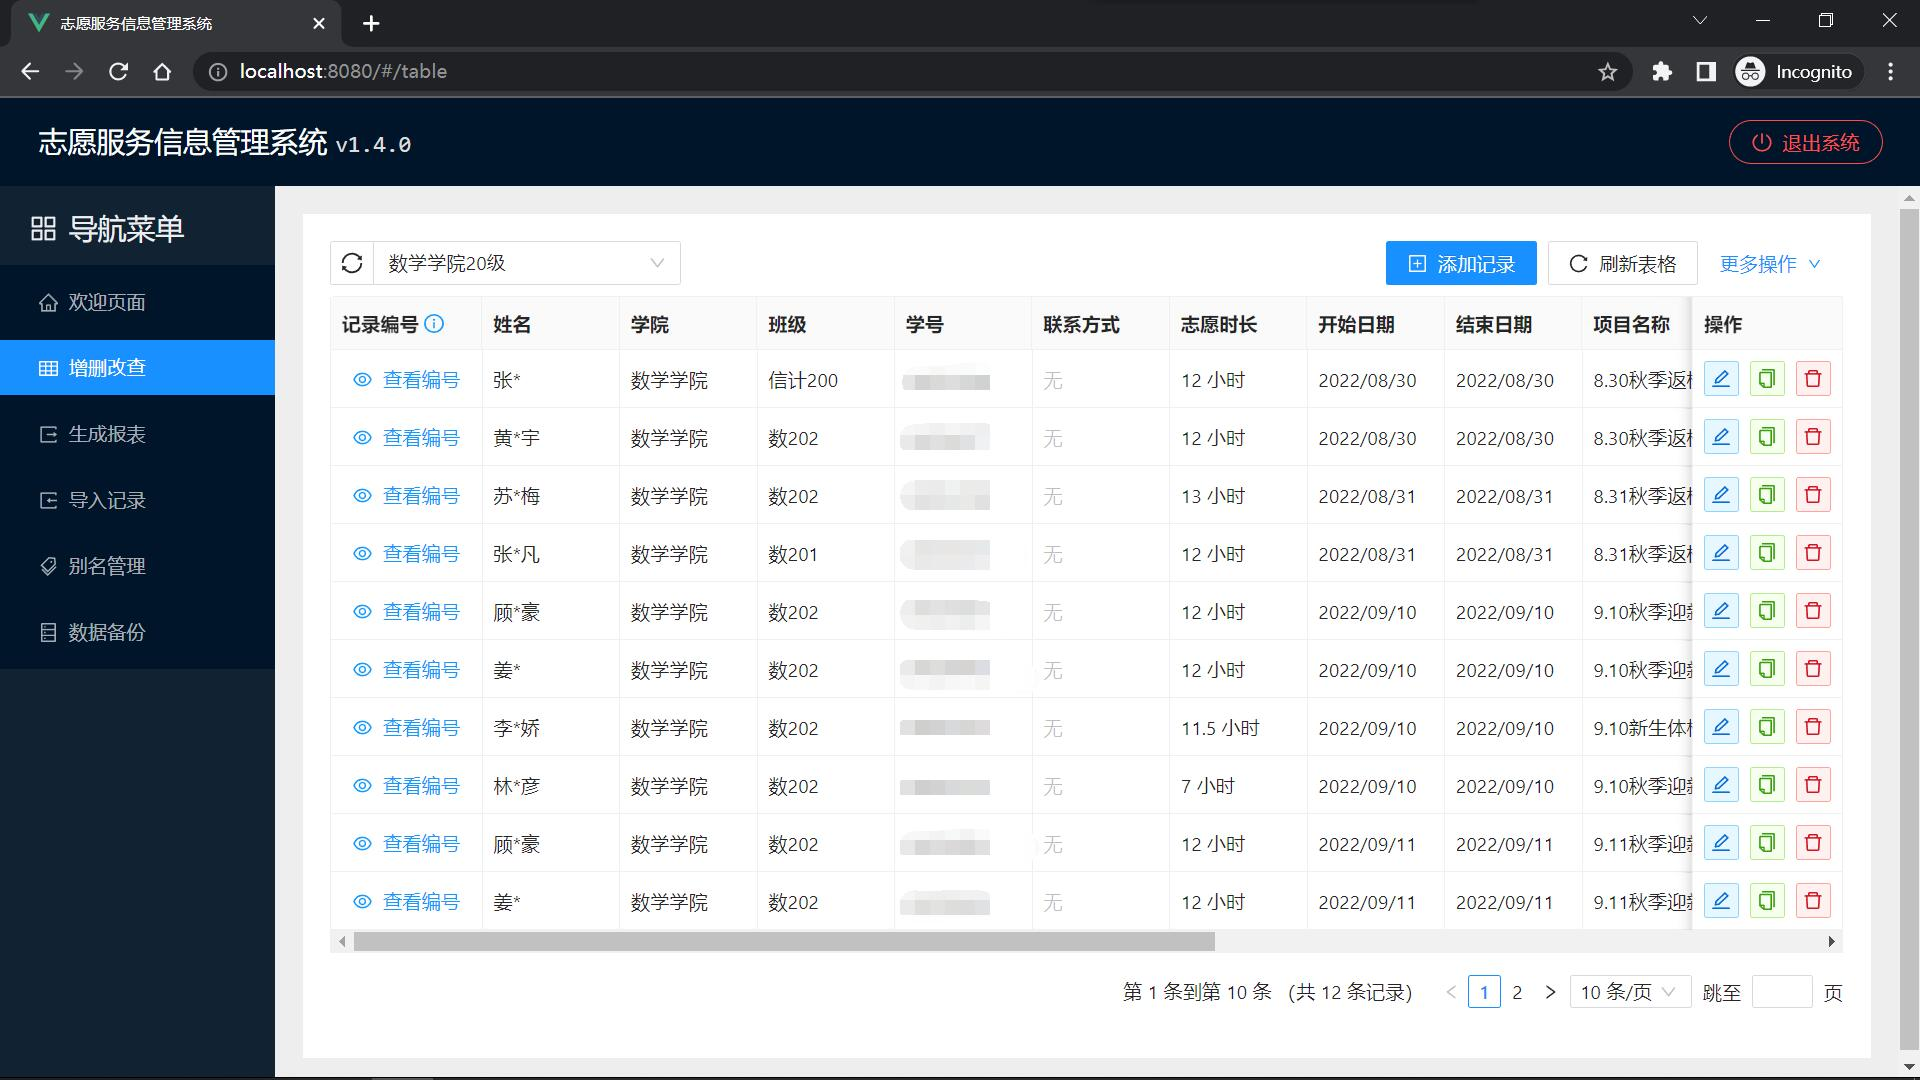
\includegraphics[width=\textwidth]{../screenshots/table.jpg}
    \caption{增删改查}
\end{figure}

录入同一活动的多条记录时,可勾选“批量导入模式”。
在此模式下,成功添加记录后不会立即清除并关闭录入表单,
而是会留在表单界面,并且保留活动信息、仅清除志愿者信息,方便连续录入。

\begin{warnings}
    \item 遇到除编号外完全相同的重复记录时,后台程序会自动忽略多余记录,仅保留第一条。
    如果确实需要导入相似数据,请填写不同的备注加以区分。
\end{warnings}

\subsection{生成报表}

在“生成报表”页面中,可以导出各种分级表格。目前,可以选择以下导出等级:

\begin{figure}[htbp]
    \centering
    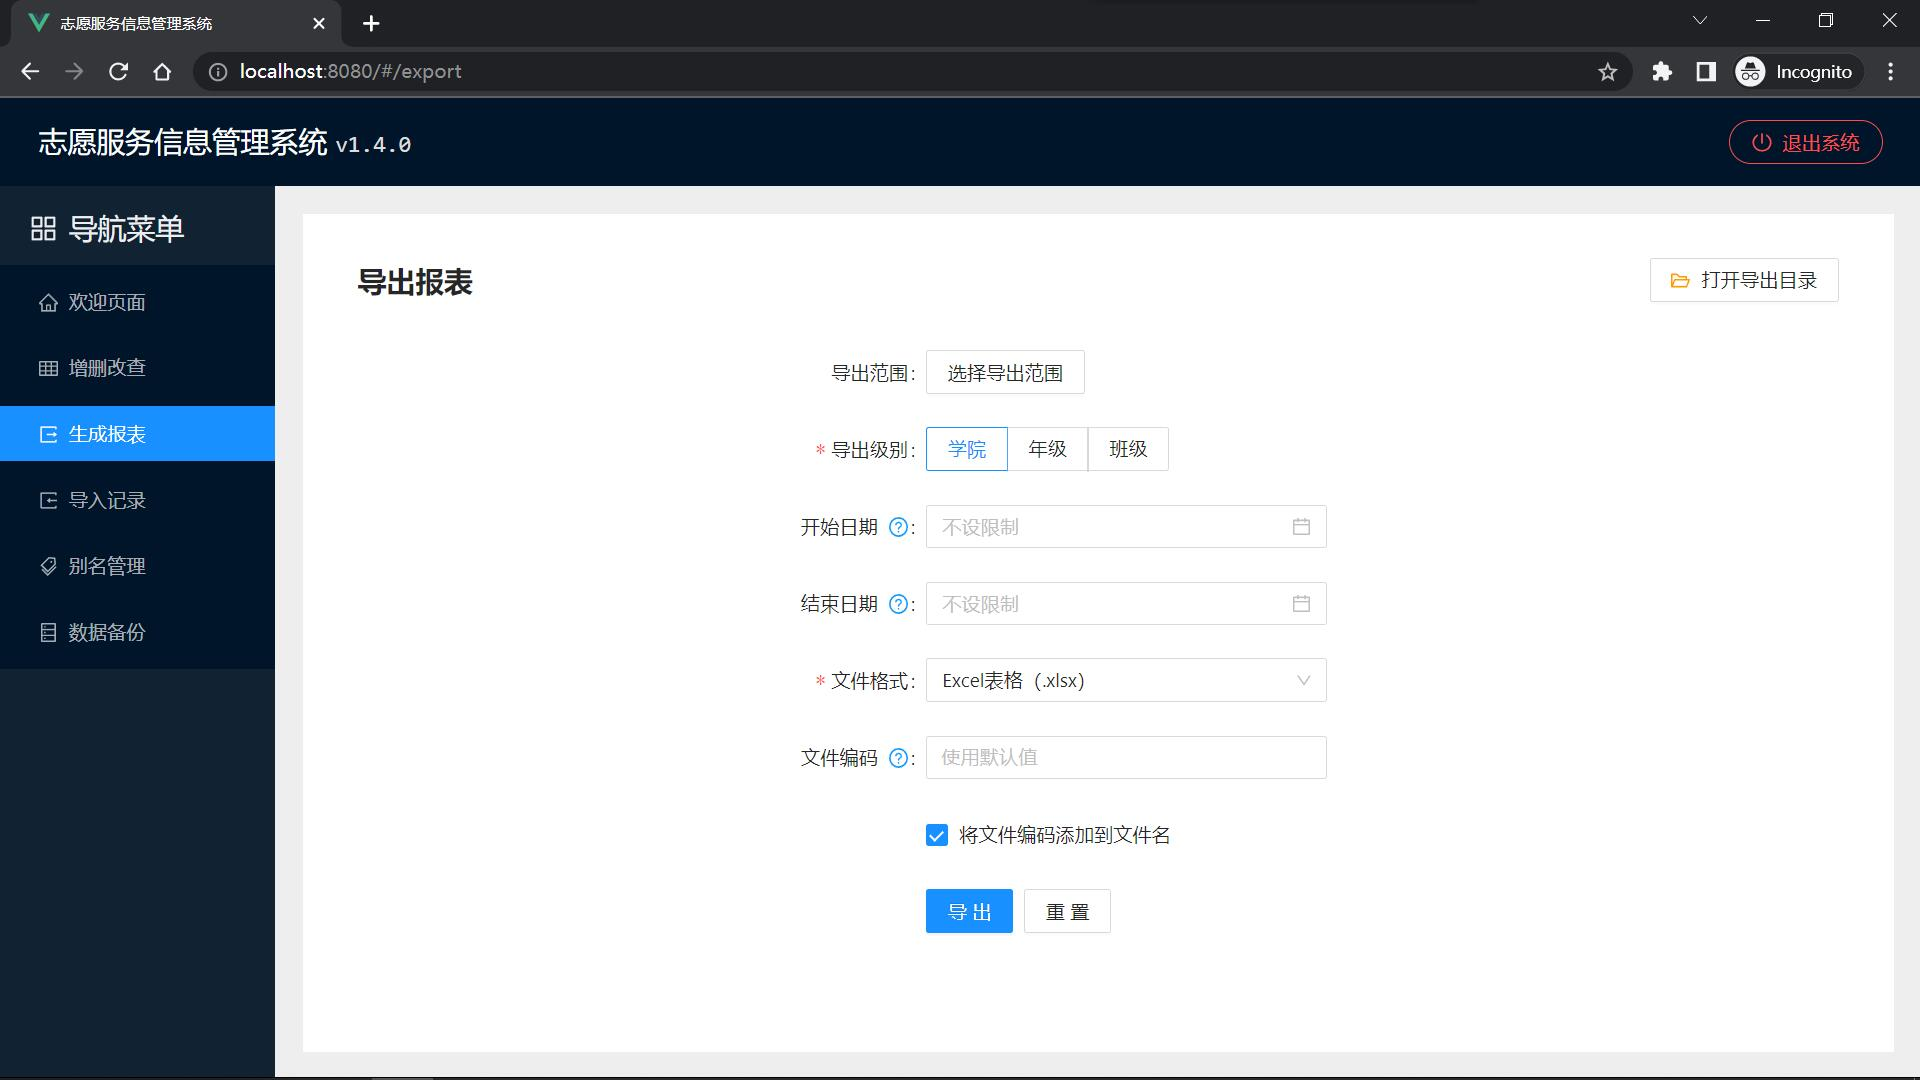
\includegraphics[width=\textwidth]{../screenshots/export.jpg}
    \caption{生成报表}
\end{figure}

\begin{description}
    \item[学院] 分学院导出数据表格,表格将以学院名称命名。
    \item[年级] 分学院和年级导出数据表格,表格将以年级命名,存放在以对应学院命名的文件夹中。
    \item[班级] 分学院、年级和班级导出表格,表格将以班级命名,存放在以对应学院和年级命名的文件夹中。
\end{description}

导出的文件(夹)会存放在软件的\texttt{export}文件夹中。
点击“生成报表”页面右上角的“打开导出目录”,后台程序会尝试在文件管理器中打开\texttt{export}文件夹。

在导出时,可以通过“导出范围”选择想要导出的数据表格,
还可以选择“开始日期”和“结束日期”对数据进行筛选。
留空则表示跳过对应的筛选。日期筛选条件如下:

\begin{description}
    \item[开始日期] 仅导出活动结束日期大于等于此日期的数据。
    \item[结束日期] 仅导出活动开始日期小于等于此日期的数据。
\end{description}

\subsection{导入记录}

在“导入记录”页面中,可以上传已有的数据表格,让后台程序自动识别并导入其中的记录。
如果有现存数据需要导入系统,请使用此功能,避免逐条手动输入。

\begin{figure}[htbp]
    \centering
    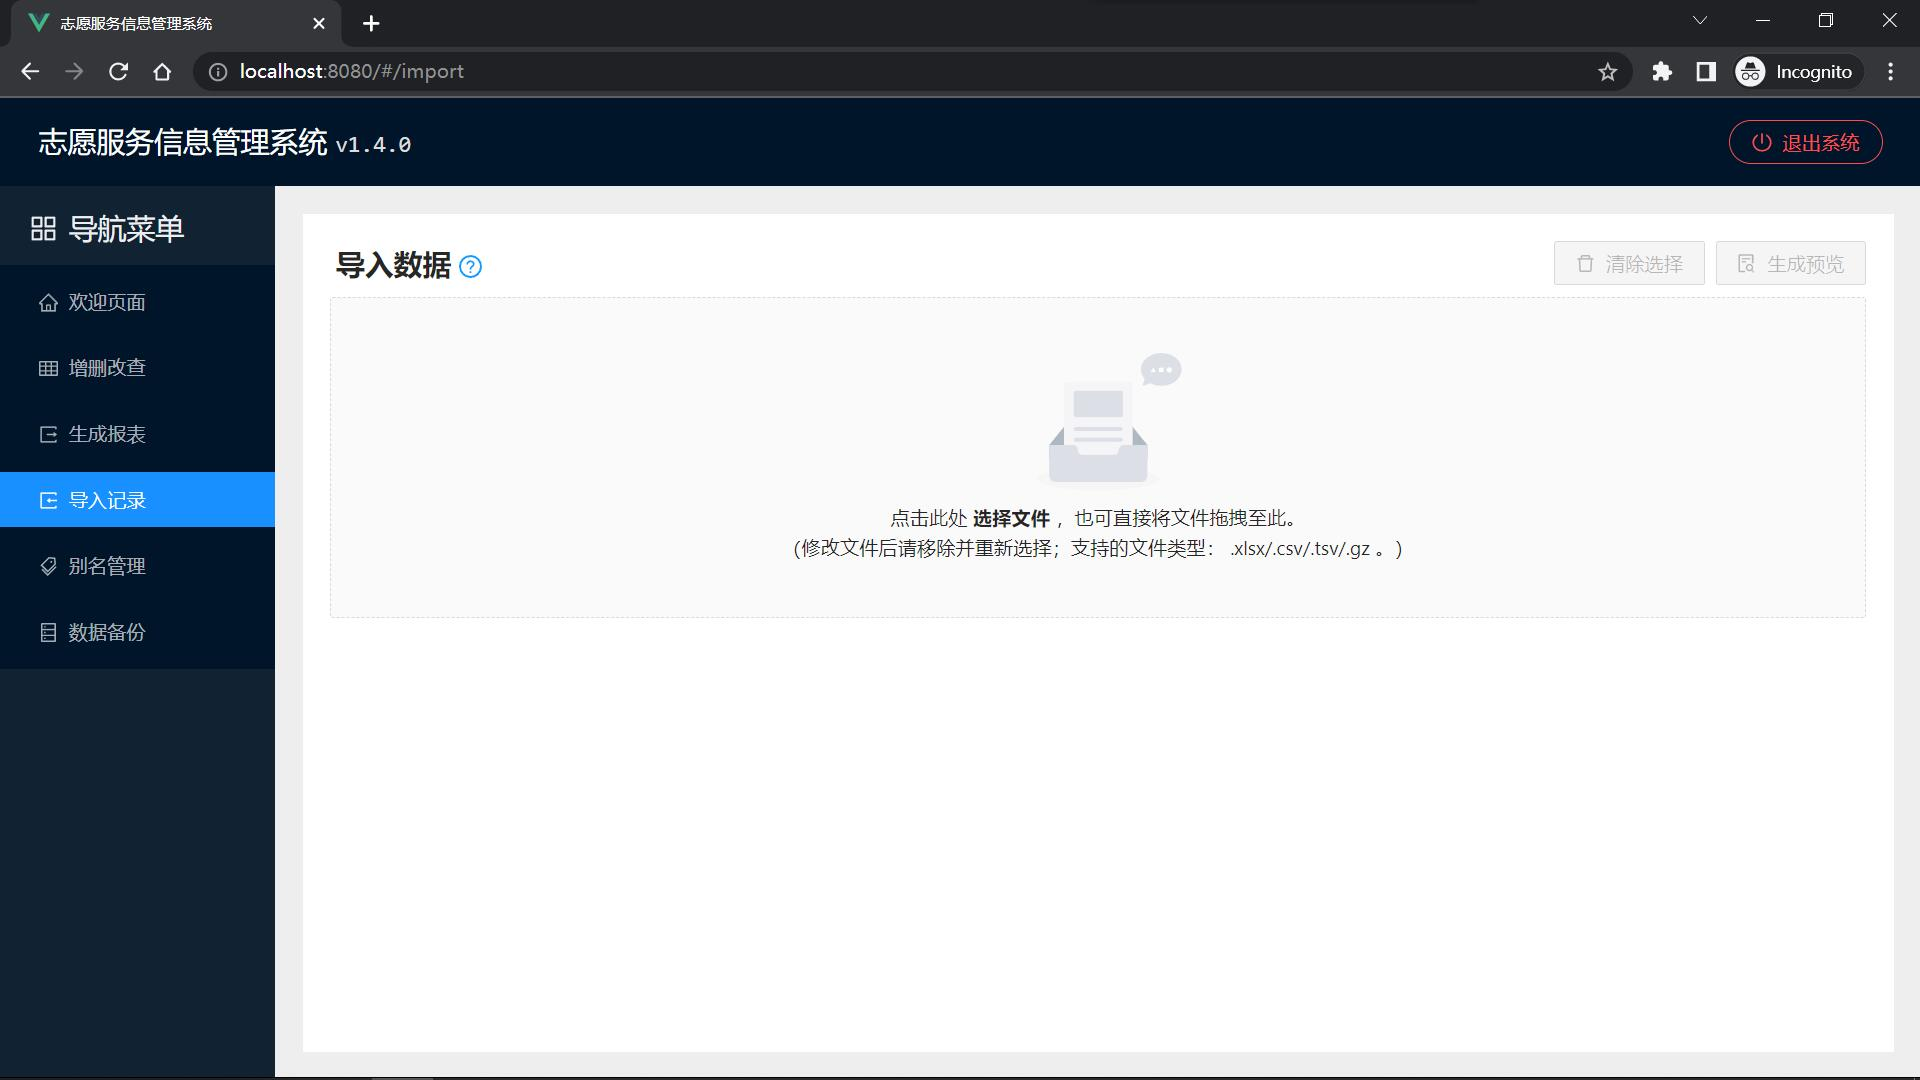
\includegraphics[width=\textwidth]{../screenshots/import.jpg}
    \caption{导入记录}
\end{figure}

导入步骤如下:

\begin{enumerate}
    \item 点击文件上传区域选择需要导入的表格文件,或直接将文件拖入此区域。
          (可以一次性选择、导入多个表格文件。)
    \item 选择好文件后,点击右上角“生成预览”。后台程序会尝试识别上传的数据,并生成预览数据。
          在此过程中,可能会遇到无法识别的问题,可以尝试手动修改表格中对应的数据后重试。
    \item 查看预览数据并确认无误后,点击右上角“提交导入”,进入最后的确认界面。
    \item 在确认界面中,会显示导入的整体信息和导入选项。点击“确认”后数据会正式导入。
\end{enumerate}

目前,导入程序已尽可能兼容各种内容格式,尤其是日期数据。
如果在导入时还是遇到了无法识别的问题,请先根据提示检查数据是否有误。
若是数据本身有问题,例如“6月31日”(不存在的日期)、“XX年暑假”(缺少明确日期)等,
麻烦手动修改,然后在上传列表中移除已选择的文件、重新上传并再次尝试生成导入预览。
如果数据格式没有明显问题,但是程序却无法识别,请进行反馈(见章节\ref{subsec:report})。

\begin{warnings}
    \item 在处理导入数据时,后台程序会自动去除单元格内的首尾空格,
    并根据设置处理别名(见章节\ref{subsec:alias})。
    \item 导入时,后台程序会自动忽略多余的重复记录,仅保留第一条。
    如果确实需要导入相似数据,请填写不同的备注加以区分。
\end{warnings}

\subsection{别名管理}
\label{subsec:alias}

在“别名管理”页面中,可以查看和修改别名设置。
在添加和导入数据时,程序会根据这里的设置将别名转化成原始名称。

\begin{figure}[htbp]
    \centering
    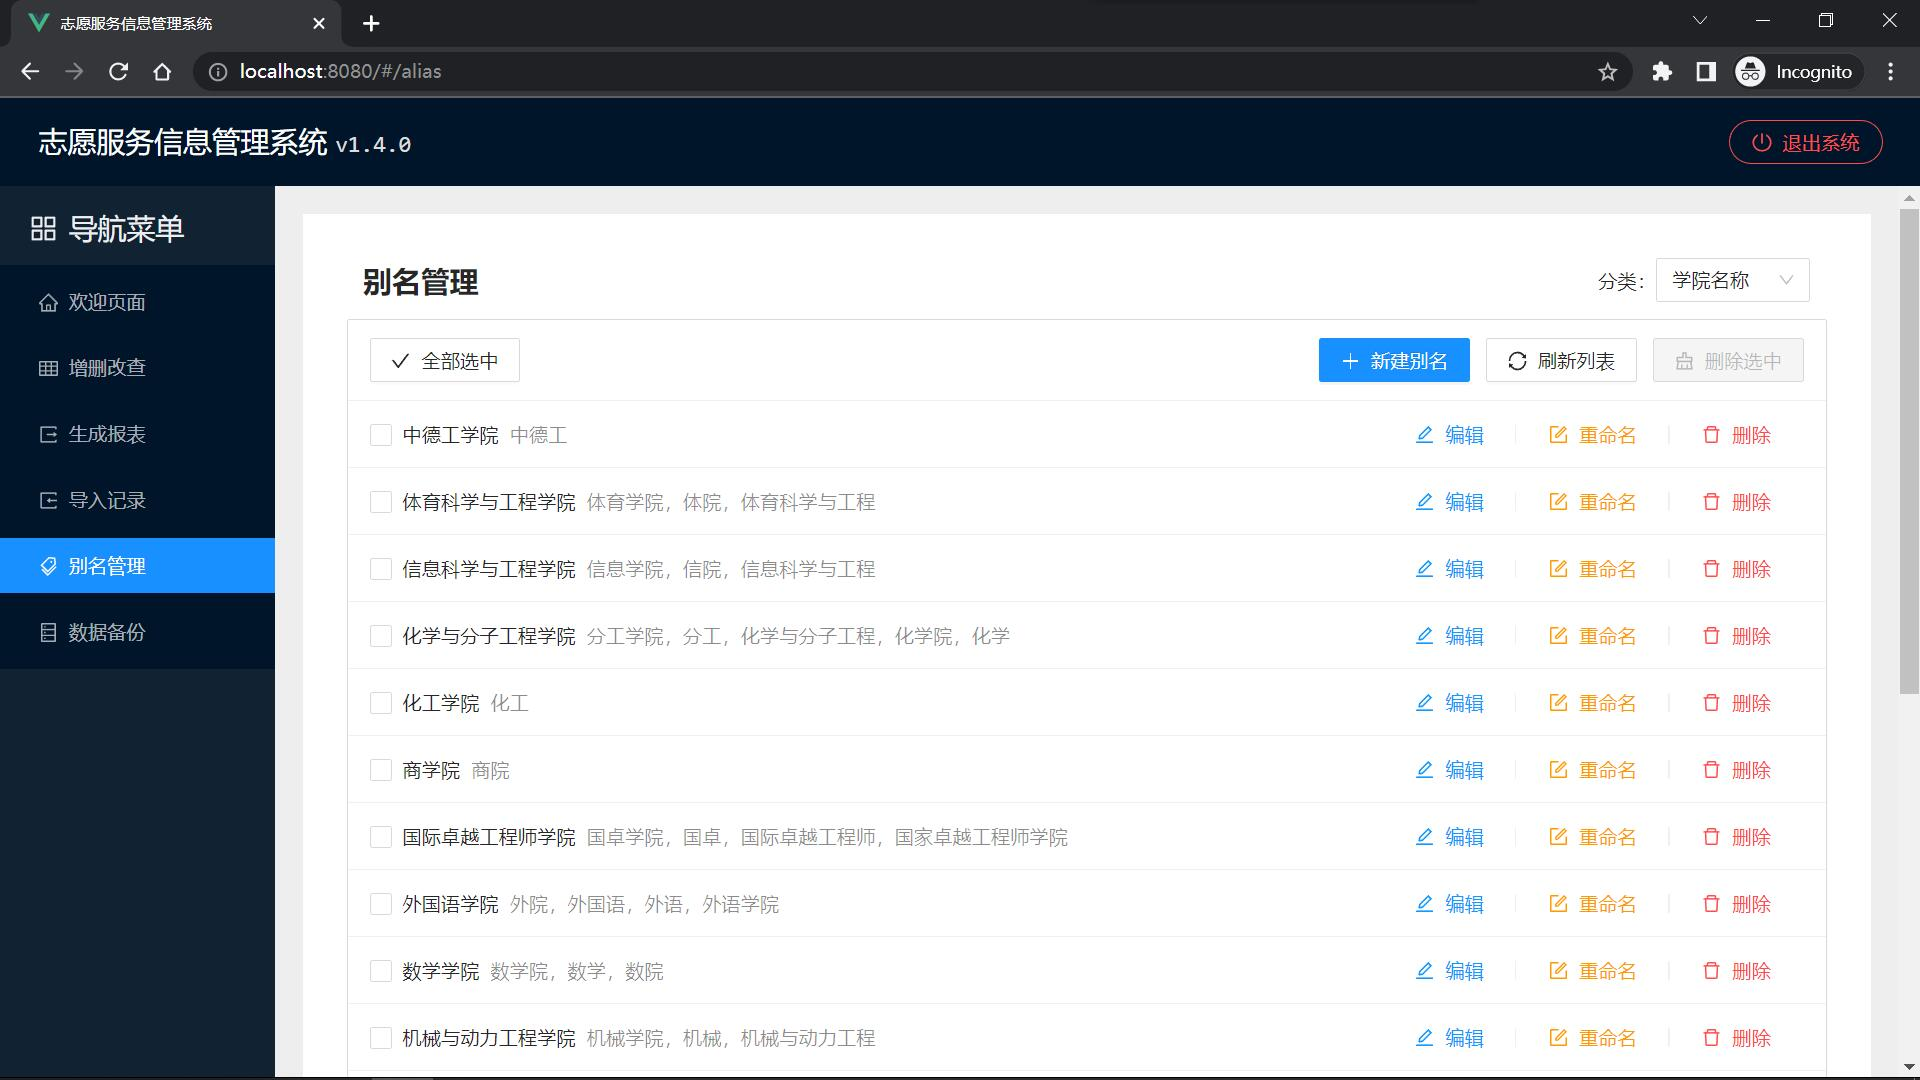
\includegraphics[width=\textwidth]{../screenshots/alias.jpg}
    \caption{别名管理}
\end{figure}

\subsection{数据备份}
\label{subsec:backup}

在“数据备份”页面中,可以查看、生成、加载和删除备份。
建议每周或每月进行一次备份,并保留最新的几次备份、删除多余备份。

\begin{figure}[htbp]
    \centering
    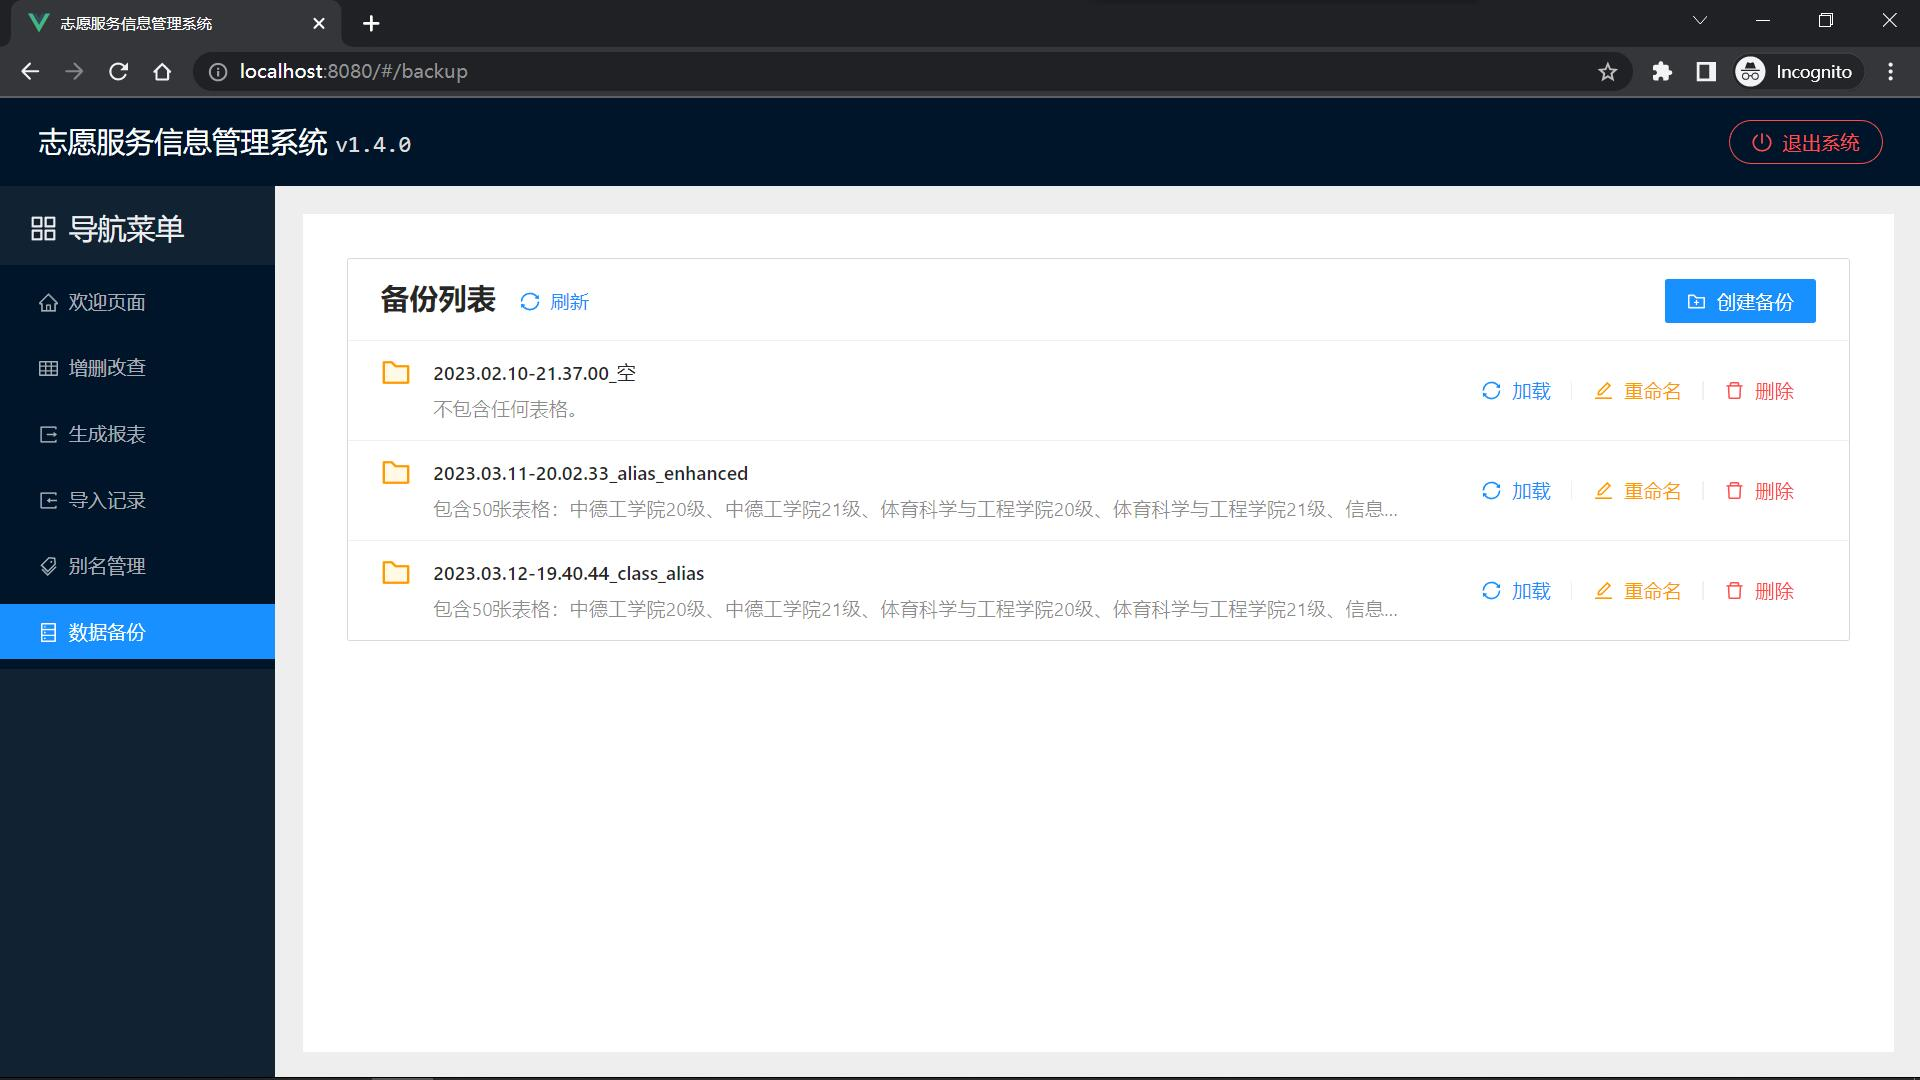
\includegraphics[width=\textwidth]{../screenshots/backup.jpg}
    \caption{数据备份}
\end{figure}

备份数据会保存在软件目录下\texttt{backup}中以备份名称命名的新文件夹里。

\begin{warnings}
    \item 加载备份不是导入数据,而是以备份数据代替当前数据。
    \item 加载备份会不可逆转地删除当前的所有数据,务必谨慎操作!
\end{warnings}

\newpage
\section{关于此软件}

\subsection{版本更新}

更新方法:

\begin{enumerate}
    \item 启动当前版本的系统,创建备份后退出。(备份方法见章节\ref{subsec:backup}。)
    \item 在\textit{GitHub Releases}\footnote{GitHub Releases: \url{\releasesurl}}
          上查找并下载新版本。
    \item 解压新版本的软件压缩包,根据新版本的使用手册初始化、启动新版系统。
    \item 在新版系统中导入第一步创建的备份数据。
          (备份数据应在旧版本软件目录下\texttt{backup}中相应的文件夹里。)
\end{enumerate}

\subsection{反馈问题}
\label{subsec:report}

如果发现软件有任何问题,欢迎在\GitHub上\href{\issuesurl}{提Issue}
\footnote{GitHub Issues: \url{\issuesurl}}。

\subsection{学习交流}

此系统为开源软件,欢迎友好的学习交流。\GitHub地址:\url{\githuburl}。

系统后端由\Python\footnote{Python官网:\url{https://www.python.org/}}
语言编写,使用\textit{Flask}\footnote{Flask官网:\url{https://flask.palletsprojects.com/}}
搭建本地服务器,借助\textit{pandas}\footnote{pandas官网:\url{https://pandas.pydata.org/}}
操作数据。

系统前端由\textit{Vite}\footnote{Vite官网:\url{https://vitejs.dev/}}
构建,主要使用\textit{Vue}\footnote{Vue官网:\url{https://vuejs.org/}}
框架和\textit{Ant Design Vue}\footnote{Ant Design Vue官网:%
    \url{https://www.antdv.com/components/overview}}
组件库。

此文档使用\LaTeX\footnote{\LaTeX官网:\url{https://latex-project.org/}}排版。

\end{document}
